\chapter{Usage Scenarios}
\section{Usage Scenarios}
MPI\_T in combination with the TAU plugin architecture makes it possible to do powerful operations that would be difficult to realize otherwise. The following describes the design of a recommendation to enable hardware offloading of collectives, and an autotuning policy to free unused MPI internal buffers using MPI\_T. These policies are implemented using plugins.
\subsection{Recommendation Use Case: Hardware Offloading of Collectives}
MVAPICH2 now supports offloading of \verb+MPI_Allreduce+ to network hardware using the SHArP~\cite{SHARP} protocol. Hardware offloading is mainly beneficial to applications where communication is sensitive to latency. As the \verb+MPI_Allreduce+ call in MiniAMR involves messages of 8 bytes, it is a prime candidate to benefit from hardware offloading. \par
During the profiling phase, TAU collects statistics about the average message size involved in \verb+MPI_Allreduce+ operation. It also collects the time spent within \verb+MPI_Allreduce+ versus the overall application time. If the message size is below a certain threshold and the percentage of total runtime spent within \verb+MPI_Allreduce+ is above a certain threshold, through \verb+ParaProf+, TAU recommends the user to set the CVAR \verb+MPIR_CVAR_ENABLE_SHARP+ for subsequent runs. Note that this recommendation policy was implemented using plugins. The same infrastructure can be used to support multiple recommendation policies.
\subsection{Autotuning Use Case: Freeing Unused Buffers}
MVAPICH2 uses internal communication buffers (VBUFs) to temporarily hold messages that are yet to be transferred to the receiver in point-to-point communications. There are multiple VBUF pools which vary in size of the VBUF. At runtime, MVAPICH2 performs a match based on the size of the message and accordingly selects a VBUF pool to use. Specifically, these VBUFs are used when MVAPICH2 chooses to send the message in an \emph{Eager} manner to reduce communication latency. Typically, short messages are sent using the \emph{Eager} protocol, and longer messages are sent using the \emph{Rendezvous} protocol, which does not involve the use of VBUFs. The primary scalability issue with using \emph{Eager} protocol is excessive memory consumption that can potentially lead to an application crash. \par
Depending on the pattern of message sizes involved in point-to-point communication, the usage level of these VBUF pools can vary with time and between processes. It can be the case that the application makes scarce use of VBUFs, or uses VBUFs only from one pool (3DStencil is one such use case). In such a scenario, unused VBUFs represent wasted memory resource. There could be significant memory savings in freeing these unused VBUFs.

For this use case, specific CVARs include:
\begin{itemize}
  \item \verb+MPIR_CVAR_IBA_EAGER_THRESHOLD+: The value of this CVAR represents the message size above which MVAPICH2 uses the \emph{Rendezvous} protocol for message transfer in point-to-point communication. Below this message size, MVAPICH2 uses the \emph{Eager} protocol
  \item \verb+MPIR_CVAR_VBUF_TOTAL_SIZE+: The size of a single VBUF. For best results, this should have the same value as \verb+MPIR_CVAR_IBA_EAGER_THRESHOLD+
  \item \verb+MPIR_CVAR_VBUF_POOL_CONTROL+: Boolean value that specifies if MVAPICH2 should try to free unused VBUFs at runtime. By default, MVAPICH2 will try to free from any available pool if this variable is set
  \item \verb+MPIR_CVAR_VBUF_POOL_REDUCED_VALUE+: This CVAR specifies the lower limit to which MVAPICH2 can reduce the number of VBUFs. This is an array, and each index represents the corresponding VBUF pool. This CVAR takes effect only if  pool control is enabled. This CVAR allows more fine-grained control over freeing of VBUFs, potentially reducing unnecessary allocations and freeing of VBUFs, if the usage pattern is known in advance
\end{itemize}

Correspondingly, PVARs of interest include:
\begin{itemize}
  \item \verb+mv2_vbuf_allocated_array+: Array that represents the number of VBUFs allocated in a pool specified by an index
  \item \verb+mv2_vbuf_max_use_array+: Array that represents the maximum number of VBUFs that are actually used in a given pool specified by an index
  \item \verb+mv2_total_vbuf_memory+: Total VBUF memory (in bytes) used for the specified process across all pools
\end{itemize}

\subsubsection{Autotuning Policy}
When we increase the value of the \emph{Eager} limit specified by \\\verb+MPIR_CVAR_IBA_EAGER_THRESHOLD+, there is an opportunity for increased overlap between communication and computation as larger messages are sent eagerly. As a result, the overall execution time for the application may reduce. Figure \ref{fig:beforeeager} is an enlarged Vampir~\cite{Vampir} summary process timeline view for one iteration of the 3DStencil application before applying the Eager optimization. Figure \ref{fig:aftereager} is a Vampir summary process timeline view for one iteration of the 3DStencil application after applying the Eager optimization. The timeline view focuses on the phase of the iteration where there is an explicit opportunity for communication-computation overlap through the use of non-blocking sends and receives. The X-axis represents time and the Y-axis represents the percentage of MPI processes inside user code (green) and MPI code (red) respectively at any given instant in time --- larger areas of green indicates a higher amount of useful work (computation) performed by processes as a result of a larger communication-computation overlap. 

 \begin{figure*}[tbp!]
  \centering
  \captionsetup{justification=centering}
  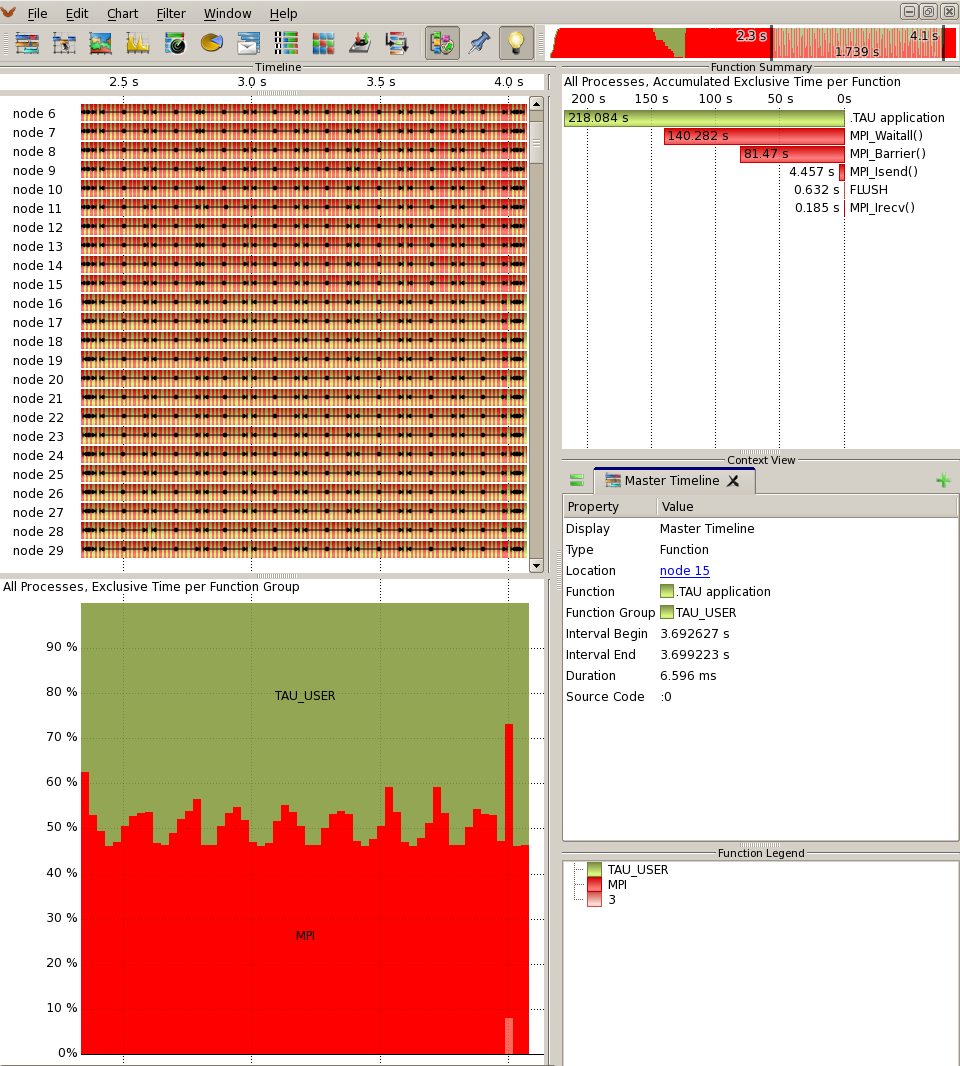
\includegraphics[scale=1.0,width=\columnwidth,keepaspectratio]{figures/Overlap-before}
         \caption{Vampir~\cite{Vampir} summary process timeline view of 3DStencil before Eager threshold tuning}
 \label{fig:beforeeager}
 \end{figure*}

 \begin{figure*}[tbp!]
  \centering
  \captionsetup{justification=centering}
  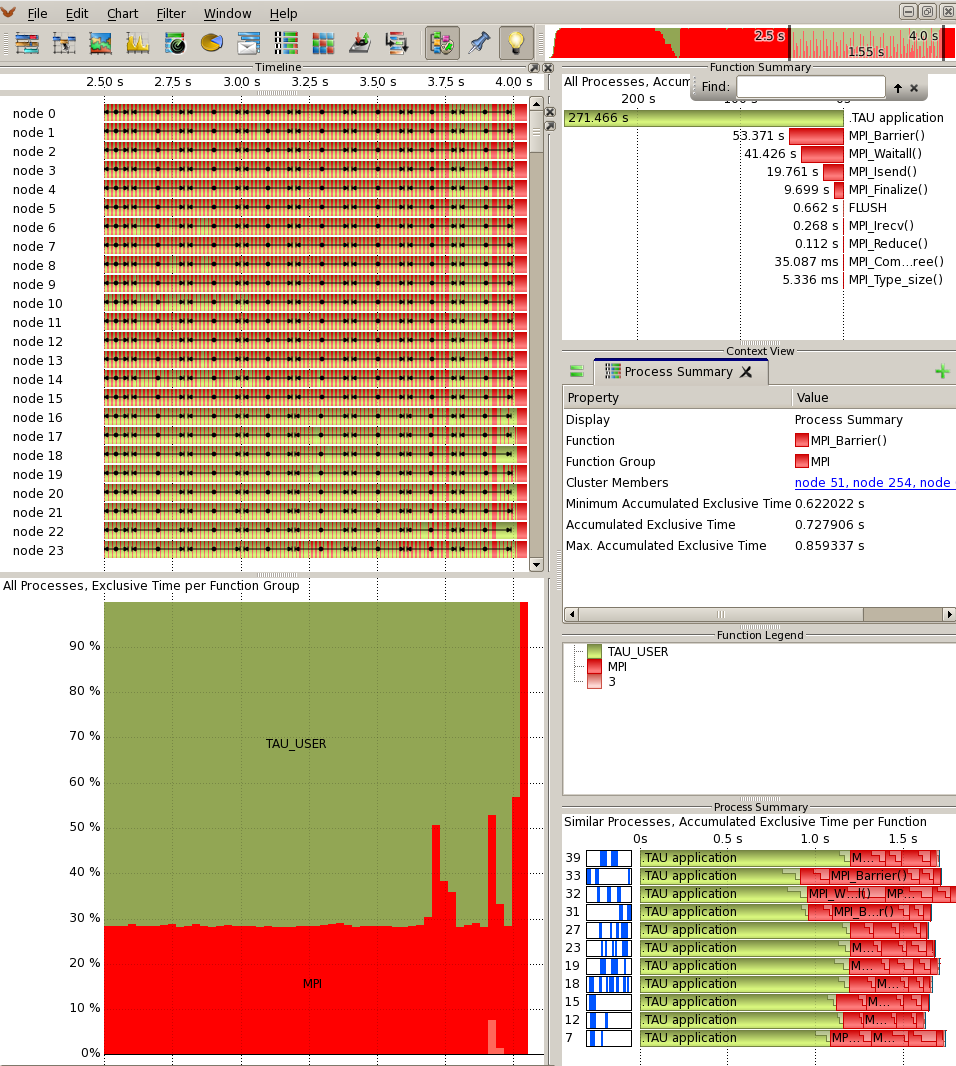
\includegraphics[scale=1.0,width=\columnwidth,keepaspectratio]{figures/Overlap-after}
         \caption{Vampir~\cite{Vampir} summary process timeline view of 3DStencil after Eager threshold tuning: Increased time spent in user code}
 \label{fig:aftereager}
 \end{figure*}


\par Figure \ref{fig:aftereager} shows the effect of an increased Eager threshold --- a 20\% increase in the number of MPI processes inside user code during the phase where communication is overlapped with computation. This increase is due to the fact that less time is spent waiting for the non-blocking calls to complete at the \verb+MPI_Wait+ barrier. With a larger eager threshold, the MPI library can advance communication in the background while the sending process is busy performing the computation. The extreme right edges of Figure \ref{fig:aftereager} are to be ignored as they represent the phase where the application is performing pure communication (refer to Section 4.4.2).\par
Increasing the Eager limit may have the following two distinct effects:
\begin{itemize}
\item Larger VBUFs may need to be allocated. Note that this does not mean that \textit{more} VBUFs are allocated --- it only means that the size of each individual VBUF in the affected pool has increased in order to hold larger messages. Recall that MVAPICH2 has four VBUF pools --- the VBUFs from different pools vary in only their size. 
\item As a result of the increased Eager limit, larger messages would be transferred through the Eager protocol instead of the Rendezvous protocol. Depending on the communication characteristics of the application, this may lead to increased usage of VBUFs from one or more VBUF pools. If there is a shortage of VBUFs in a given pool, MVAPICH2 may need to allocate additional VBUFs.
\end{itemize}
A combination of these two factors may lead to an increase in the total VBUF memory usage inside MVAPICH2. Figure \ref{fig:pycoolrincr} is a PYCOOLR screenshot illustrating this increase in total VBUF memory usage (across all four pools) for AmberMD application when the Eager threshold is raised. We see a similar increase in total VBUF memory usage for the 3DStencil application as well. The X-axis represents time and the Y-axis represents memory in bytes with 10\textsuperscript{7} as the multiplier. Each red dot represents the instantaneous \verb+mv2_total_vbuf_memory+ (in bytes) for one MPI process. If MPI processes have the same VBUF memory usage at any point in time, then the red dots would overlap. From Figure \ref{fig:pycoolrincr}, it is evident that there are two classes of processes --- one with a VBUF memory usage of roughly 3 MB (before Eager tuning), and another with a VBUF memory usage level of roughly 6 MB (before Eager tuning). The eager threshold is raised by setting the CVAR \verb+MPIR_CVAR_IBA_EAGER_THRESHOLD+ and \verb+MPIR_CVAR_VBUF_SIZE+ statically, during \verb+MPI_Init+. Figure \ref{fig:pycoolrincr} shows that the \verb+mv2_total_vbuf_memory+ increases to approximately 12 MB for the processes with a lower VBUF memory usage, and approximately 23 MB for the class of processes with a higher VBUF memory usage. \par 
